\documentclass[a4paper, 12pt]{book}
% preamble.tex

\usepackage[utf8]{inputenc}
\usepackage[T1]{fontenc}
\usepackage[english]{babel} % Ho cambiato in italian, supponendo che la maggior parte del testo sia in italiano
\usepackage{amsmath}
\usepackage{amssymb}
\usepackage{graphicx}
\usepackage{hyperref}
\usepackage{geometry}
\usepackage{fontspec} % Utile per Xetex/LuaLaTeX ma mantenuto
\usepackage{booktabs}
\usepackage{amsthm}
\usepackage{enumitem}
\usepackage{caption}
\usepackage{thmtools}
\usepackage{standalone} % Già presente nel tuo elenco
\usepackage{tkz-euclide}
\usepackage{graphicx}
\usepackage[T1]{fontenc}
\usepackage{wesa}

% --- PACCHETTI AGGIUNTI PER LA FORMATTAZIONE ---
\usepackage{parskip}  % Aggiunge spazio tra i paragrafi (stile "blocco")
\usepackage{fancyhdr} % Per intestazioni e piè di pagina personalizzati

% --- IMPOSTAZIONI GEOMETRIA E FONT ---
\geometry{a4paper, margin=1in}

% Configura lo stile 'plain' (usato da \maketitle e \tableofcontents)
% per essere coerente con il piè di pagina
\fancypagestyle{plain}{
    \fancyhf{} % Pulisce
    \cfoot{\thepage} % Mette solo il numero di pagina
    \renewcommand{\headrulewidth}{0pt} % Niente linea su queste pagine
}

% Configurazione Header/Footer per le altre pagine
\pagestyle{fancy}
\fancyhead{} % Pulisce l'intestazione
\fancyfoot{} % Pulisce il piè di pagina
\fancyhead[L]{\nouppercase{\rightmark}} % Nome Sezione a sinistra (o Chapter)
\fancyhead[R]{\nouppercase{\leftmark}}  % Nome Capitolo a destra (o Sezione)
\fancyfoot[C]{\thepage} % Numero di pagina al centro
\renewcommand{\headrulewidth}{0.4pt}
\renewcommand{\footrulewidth}{0pt}


% --- DEFINIZIONI TEOREMI ---
% (Questa parte è cruciale per la tua struttura)
\newtheoremstyle{mythmstyle}%
    {}%
    {}%
    {\itshape}%
    {}%
    {\bfseries}%
    {}%
    { }%
    {\thmname{#1}\thmnumber{ #2}%
    \thmnote{: #3\addcontentsline{toc}{subsubsection}{{\itshape#1}: #3}}. }

% 2. Imposta questo stile come quello ATTUALE
\theoremstyle{mythmstyle}

\newtheorem{theorem}{Th}[section]
\newtheorem{definition}{Def}[section]
\newtheorem{proposition}{Prop}[section]
\newtheorem{corollary}{Cor}[section]
\newtheorem{algorithm}{Alg}[section]
\newtheorem{lemma}{Lemma}[section]
\newtheorem*{remark}{Rem}

% Definizioni utili per il Main file
\newcommand{\inputlesson}[1]{\clearpage\input{#1}\clearpage} % Comando per input lezione

\usepackage{tikz}
\usetikzlibrary{shapes,fit}
\usepackage{pgfplots}
\pgfplotsset{compat=1.18}
\usepackage{amsmath} % Required for align environment
\usepackage{caption} % Required for \captionof outside float environments



\begin{document}
\setcounter{chapter}{11}
\chapter{Lesson 10-12-2025}
\section{Space correlation}

\subsection{About space correlation (dependance of \texorpdfstring{$y$}{y} on \texorpdfstring{$\theta$}{θ}, arrival angle); specialization for when \texorpdfstring{$x$}{x} is sinusoidal}

Let's suppose the \textbf{transmitter is fixed}. Let's study the fading dynamics as a function of the position of the receiver: in other words, let's see what happens if the receiver moves during the transmission.

\begin{yellowbox}
\faBook\ \textit{Channel modeling (pp. 131-208), page 19}

The simultaneous dependence on the positions of both transmitter and receiver, essential for MIMO channel modeling, is deferred to later in the chapter.
\end{yellowbox}

We transmit a signal $x$ which experiences a delay depending on $D(\theta)$, difference in path length depending on the angle: the experienced delay will thus be $D(\theta)/c$.

\begin{center}
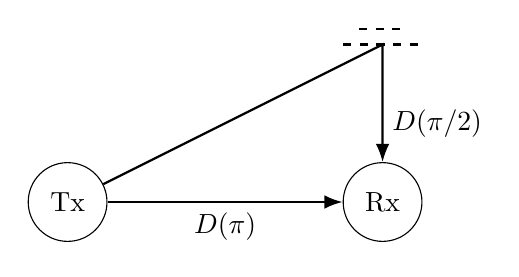
\begin{tikzpicture}[scale=1.0, >=Latex]
    % Nodes Tx and Rx
    \node[draw, circle, minimum size=1cm] (Tx) at (0,0) {Tx};
    \node[draw, circle, minimum size=1cm] (Rx) at (4,0) {Rx};

    % Straight path D(pi)
    \draw[->, thick] (Tx) -- (Rx) node[midway, below] {$D(\pi)$};

    % Angled path
    % Trying to replicate the triangle shape in the image
    \coordinate (Top) at (4, 2); % The arrow points to Rx from top
    \draw[->, thick] (Tx) -- (Top) -- (Rx);
    
    % Dashed lines at top
    \draw[dashed, thick] (3.5, 2) -- (4.5, 2);
    \draw[dashed, thick] (3.7, 2.2) -- (4.3, 2.2); % Stacked dashed lines
    
    % Label D(pi/2)
    \node[right] at (4, 1) {$D(\pi/2)$};

\end{tikzpicture}
\end{center}

\begin{greenbar}
Simple illustration showing what we mean by $D(\theta)$.
\end{greenbar}

In this context in which the angle is important, we don't have an omnidirectional pattern: it's more sensitive in certain angles and less in others: this is characterized through $\mathcal{P}(\theta)$, the \textcolor{green!60!black}{PAS}; $G_r(\theta)$ is the directional gain.

We'll thus have that the \textbf{baseband noiseless signal at a given location can be expressed as}

\begin{align}
y(t) = \sqrt{G} \int_{-\pi}^{\pi} \sqrt{\mathcal{P}(\theta) G_r(\theta)} x(t - D(\theta)/c) d\theta \,. \tag{3.34}
\end{align}

\begin{center}
    \footnotesize \textcolor{blue}{\faPen\ \textit{Handwritten notes on (3.34):}} \\
    \begin{itemize}
        \item On $G_r(\theta)$: \textcolor{blue}{antenna gain is included in $G$, the pattern is normalized.}
        \item On $D(\theta)/c$: \textcolor{blue}{difference in path length as a function of angle.}
    \end{itemize}
\end{center}

\textbf{If we have that $x(t)$ is a sinusoid} (expressed as $x e^{-j\phi(t)}$ with $x$ fixed in time), \textbf{in baseband it will be constant} (i.e.: we know that the baseband representation of a signal is obtained by centering its oscillation frequency around zero; if we do so \colorbox{yellow!20}{with $e^{-j\omega t}$}, we're \colorbox{yellow!20}{sure to obtain a constant term}), of phase given by the delay $\phi(\theta) = 2\pi D(\theta)/\lambda_c$ (more about this below):

\begin{align}
y &= \sqrt{G} \int_{-\pi}^{\pi} \sqrt{\mathcal{P}(\theta)G_r(\theta)} x e^{-j\phi(\theta)} \, d\theta \tag{3.35} \\
&= \sqrt{G}x \underbrace{\int_{-\pi}^{\pi} \sqrt{\mathcal{P}(\theta)G_r(\theta)} e^{-j\phi(\theta)} \, d\theta}_{h_0} \tag{3.36} \\
&= \sqrt{G} x h_0 \,. \nonumber
\end{align}

\begin{flushright}
\small
\textcolor{red}{it is a constant, 1! why?} \\
\textcolor{black}{\textbf{Note:}} $e^{-j2\pi f_c t}$ baseband equivalent
\end{flushright}

All this turns out to be a constant, hence why we call it $h_0$; this $h_0$ depends on many things.
We don't know $\mathcal{P}(\theta)$, but it is reasonable to say that:

\begin{itemize}
    \item if we have enough paths which are independent in phase
    \item and if the PAS can be modeled as uniform
\end{itemize}

this enables us to \textbf{treat $h_0$ as a complex Gaussian variable}.

Let's say we're now not at location 0, but at location 1 (a setting of distance $\Delta_D$ from location 0 we considered from (3.34) to (3.36)), with reference to the image below.

\begin{figure}[h]
    \centering
    % [IMAGE PLACEHOLDER: Diagram of Transmitter, Scatterer, Diffraction, Reflection, Receiver 0/1]
    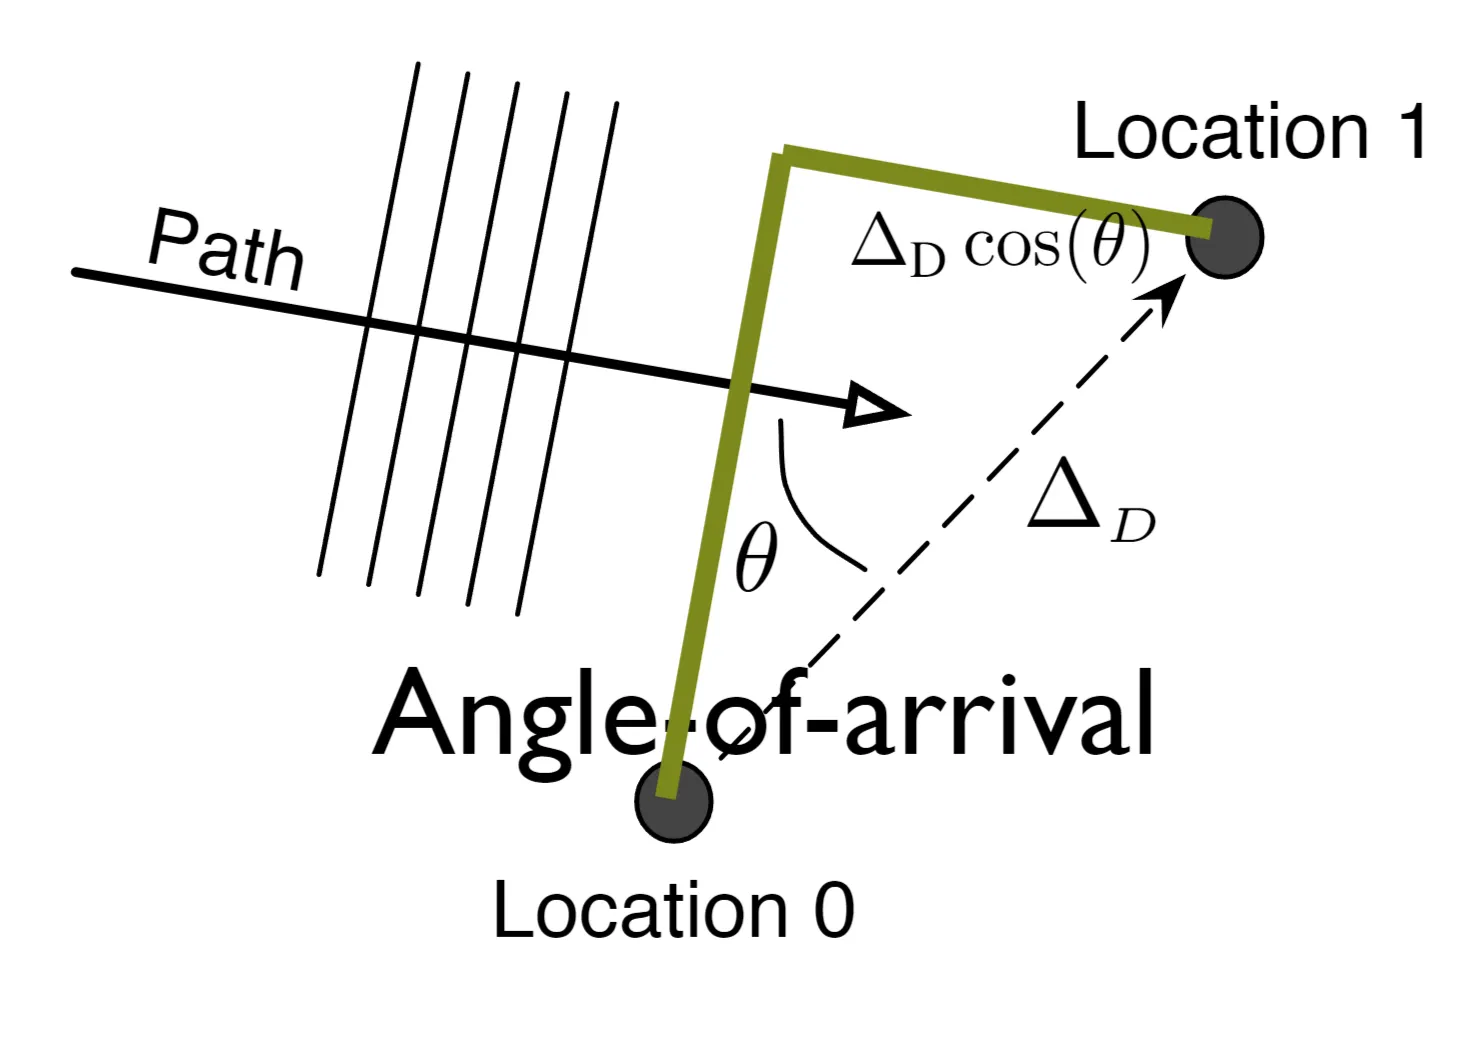
\includegraphics[width=0.5\textwidth]{Pictures/immagine-000.png}
\end{figure}

We want to find the correlation between the two received signals; we'll have (for a sinusoidal signal)

\begin{align}
h_1 = \int_{-\pi}^{\pi} \sqrt{\mathcal{P}(\theta) G_r(\theta)} \, e^{-j [\phi(\theta) + 2\pi \Delta_D \cos(\theta)/\lambda_c]} \, d\theta \,. \tag{3.38}
\end{align}

\begin{purplebox}[\faSkull \, About the phase shift]
We know the space difference between two arrival points from the point of view of a plane wave is of $\Delta_D \cos(\theta)$; we also know that the (baseband) em waves have a dependance on time through a term $e^{-j\omega t}$.

Our delay will be equal to $\Delta_D \cos(\theta)/c$, rendering the exponent as
\[
\exp\left( -j \frac{\omega_c \Delta_D \cos(\theta)}{c} \right) = \exp\left( -j \frac{2\pi c \Delta_D \cos(\theta)}{c \lambda_c} \right) \,,
\]
ultimately giving what we have in (3.38), aka a phase shift of
\[
2\pi \Delta_D \cos(\theta)/\lambda_c \,.
\]
\end{purplebox}


% Contenuto pagina 03

We can make our calculations to \textbf{find the correlation} (see 08.3 Channel modeling (pp. 131-208), page 19): we want to find it because we don't want to collect replicas of the signal; we want to have signals being collected independently so that we can process them and enjoy their independence.
If they are completely correlated, if one goes down the other will as well. If they're completely uncorrelated, if one goes down we can receive the signal at another receiver.

In the end we find that \textbf{if the phase at each angle is uniformly distributed} ($\theta \sim \mathcal{U}[-\pi, \pi)$) s.t. the expectation is nonzero only for $\theta_0 = \theta_1$), the correlation will be

\begin{align}
R_h(\Delta_D) = \mathbb{E}[h_0 h_1^*] = \int_{-\pi}^{\pi} \underbrace{\mathcal{P}(\theta) G_r(\theta)}_{\text{to be known}} e^{j 2\pi \Delta_D \cos(\theta) / \lambda_c} \, d\theta \,. \tag{3.41}
\end{align}
\begin{flushright}
\textcolor{red}{\footnotesize \textit{remember the result...}}
\end{flushright}

The antenna pattern $G_r(\cdot)$ can in principle be designed to modify the environment's PAS, and thus $R_h(\cdot)$, at the expense of failing to capture all the incoming power [239, 240].
However, the \textbf{habitual design principle} is to apply an \textbf{antenna pattern that is broader than the PAS, and approximately flat} thereupon, so as to essentially capture all of the power.
If the PAS is unknown or the antenna cannot be properly pointed, as is often the case, a uniform pattern is then preferable and (3.41) simplifies to

\begin{align}
R_h(\Delta_D) = \int_{-\pi}^{\pi} \mathcal{P}(\theta) \, e^{j 2\pi \Delta_D \cos(\theta) / \lambda_c} \, d\theta \,. \tag{3.42}
\end{align}

\begin{purplebox}[\faSkull \, How did we get rid of the double integral?]
I think that in the end we got rid of the integral mainly by assuming that $h_0, h_1$ are independent of one another if their respective signals were received from different angles; for this reason, they were only considered for $\theta_0 = \theta_1 = \theta$.
\end{purplebox}

\begin{greenbar}
Btw this last paragraph was \textcolor{ForestGreen}{from the book}
\end{greenbar}

\section{Space correlation function for Clarke-Jakes PAS}

For Clarke-Jakes PAS

With
\begin{align}
\mathcal{P}(\theta) = \frac{1}{2\pi} \quad \theta \in [-\pi, \pi) \tag{3.27}
\end{align}
, integral (3.42) gives

\begin{align}
R_h(\Delta_D) = J_0(2\pi \Delta_D / \lambda_c) \,, \tag{3.43}
\end{align}

where $J_0(\cdot)$ is the zero-order Bessel function of the first kind.

The graph of such space correlation is

\begin{figure}[h]
    \centering
    % [IMAGE PLACEHOLDER: Diagram of Transmitter, Scatterer, Diffraction, Reflection, Receiver 0/1]
    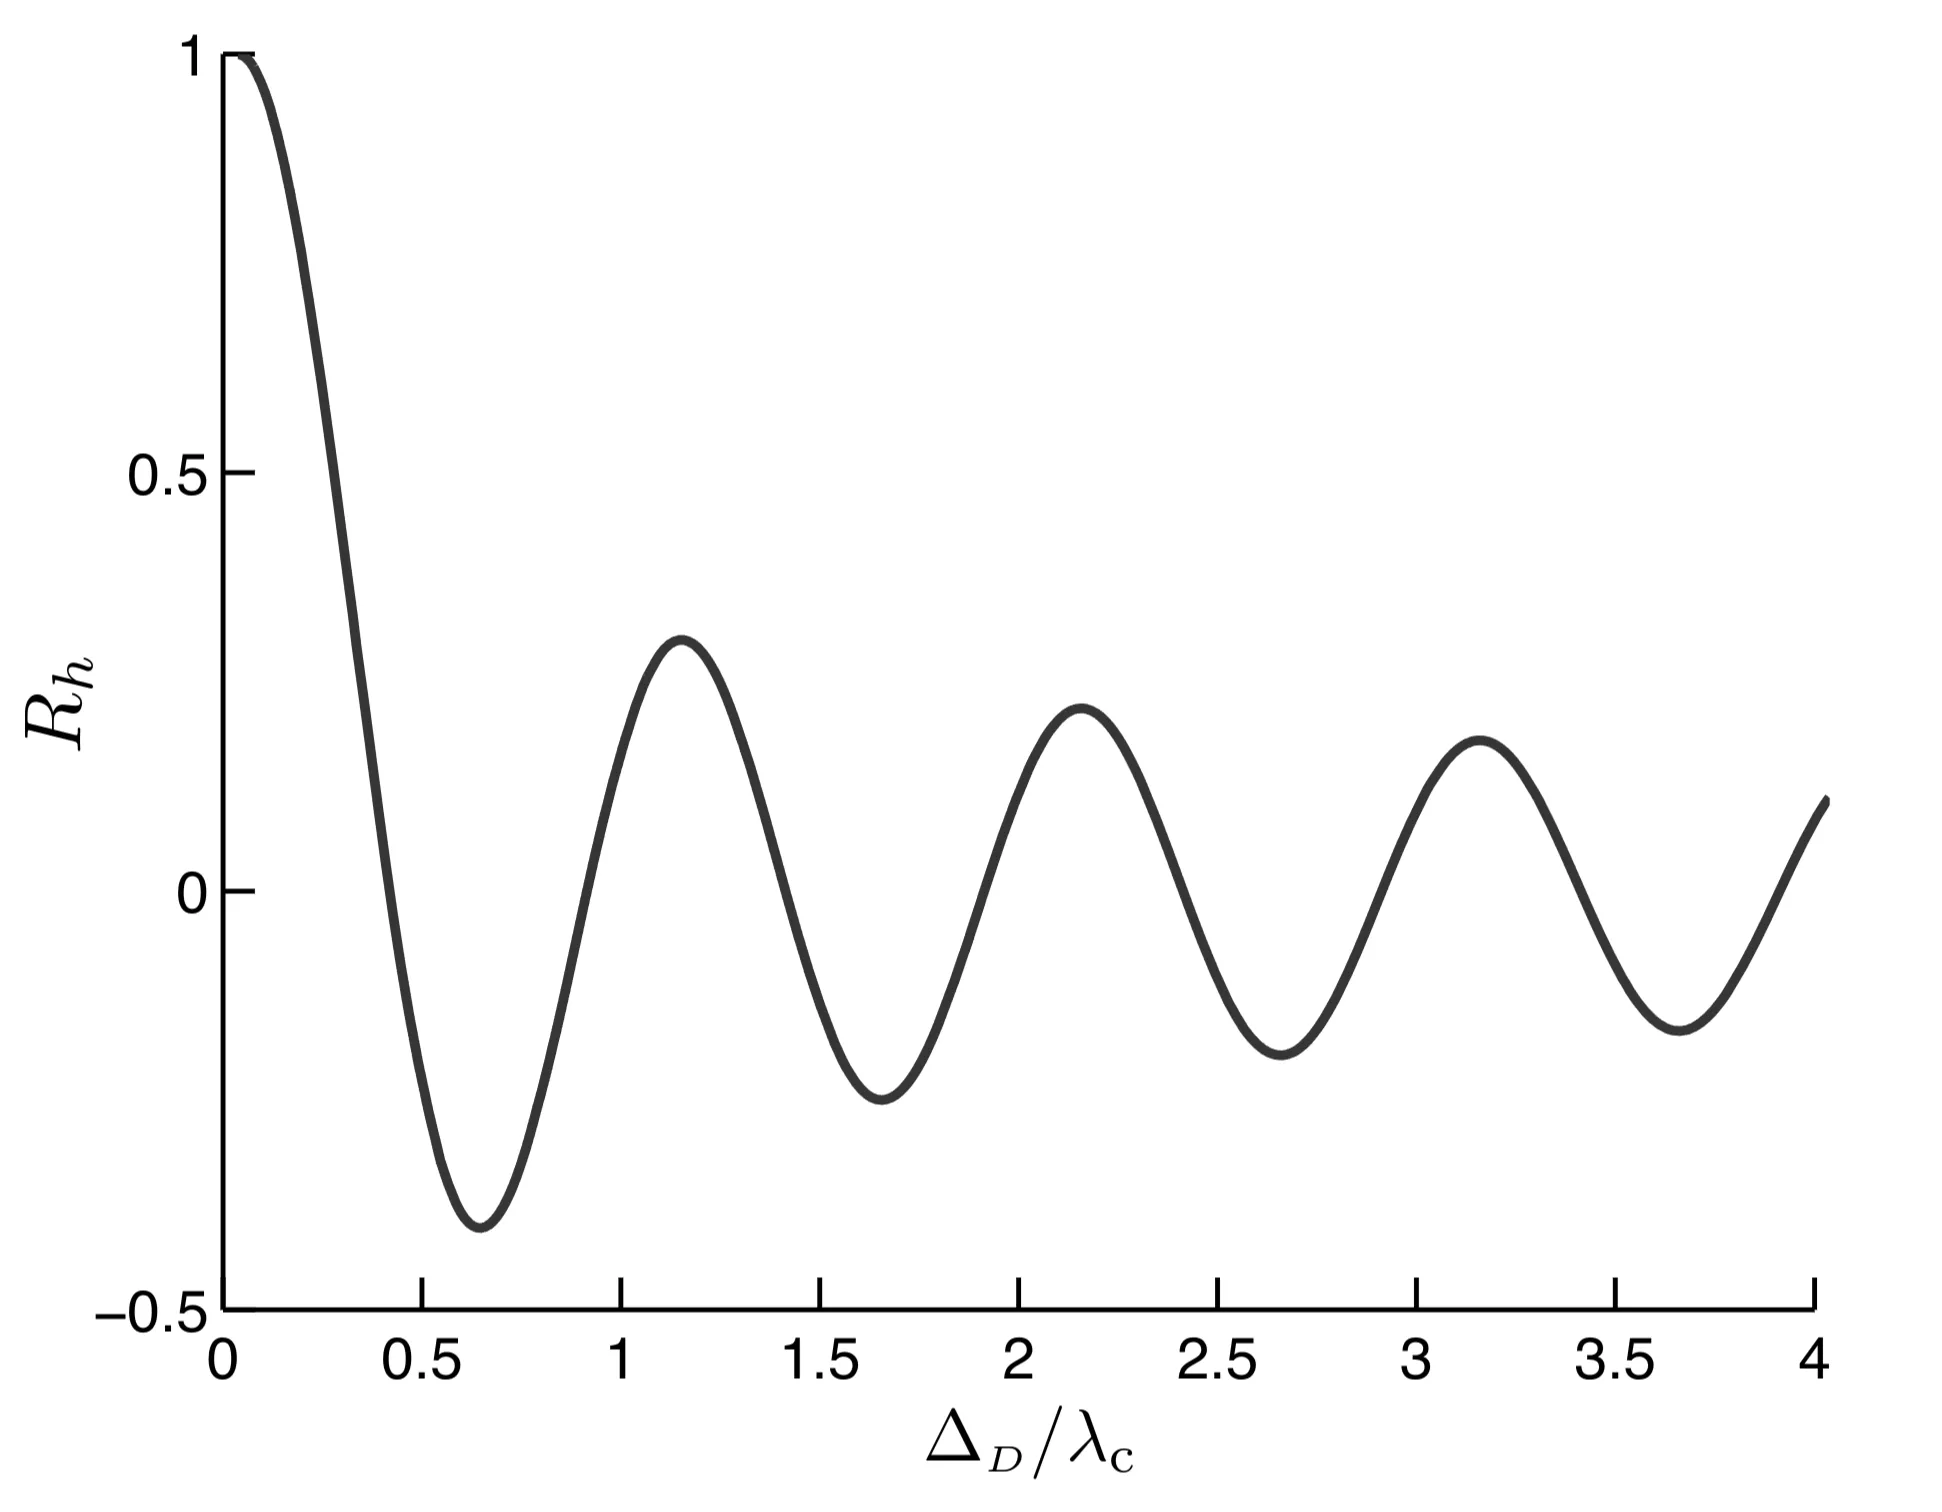
\includegraphics[width=0.7\textwidth]{Pictures/immagine-001.png}
\end{figure}

We see we cross the 0 multiple times and also that at a certain point we'll converge to 0, aka uncorrelation; this is a Bessel function of order 0.
The fact that \textbf{the first crossing of the zero happens for $D_c = 0.38\lambda_c$ is important}: it tells us how far we need to space the antennas in order to receive zero-correlation.

\begin{bluebox}[\faPen \, Coherence distance]
The mentioned value $D_c$ is the so-called \textbf{coherence distance}: it is a distance $\Delta_D$ such that $R_h(\Delta_D) = 0$; generally the value of the first crossing of 0 is considered.
This is of crucial importance when evaluating a channel, as it expresses how spaced apart two antennas should be in order for the received signals to be uncorrelated.

\begin{greenbar}
For the Clarke-Jakes, we have $D_c = 0.38\lambda_c$.
\end{greenbar}
\end{bluebox}

This is an idealized case, though. The rule of thumb is that we need to be \textbf{at least half a wavelength far away from one another}. If we want to use MIMO, we should try to have this situation; this translates to the fact that we want to have a full-rank matrix. If we want to have independent antennas, we need to space them of half a wavelength.
Really rough intuition:

\begin{figure}[h]
    \centering
    % [IMAGE PLACEHOLDER: Diagram of Transmitter, Scatterer, Diffraction, Reflection, Receiver 0/1]
    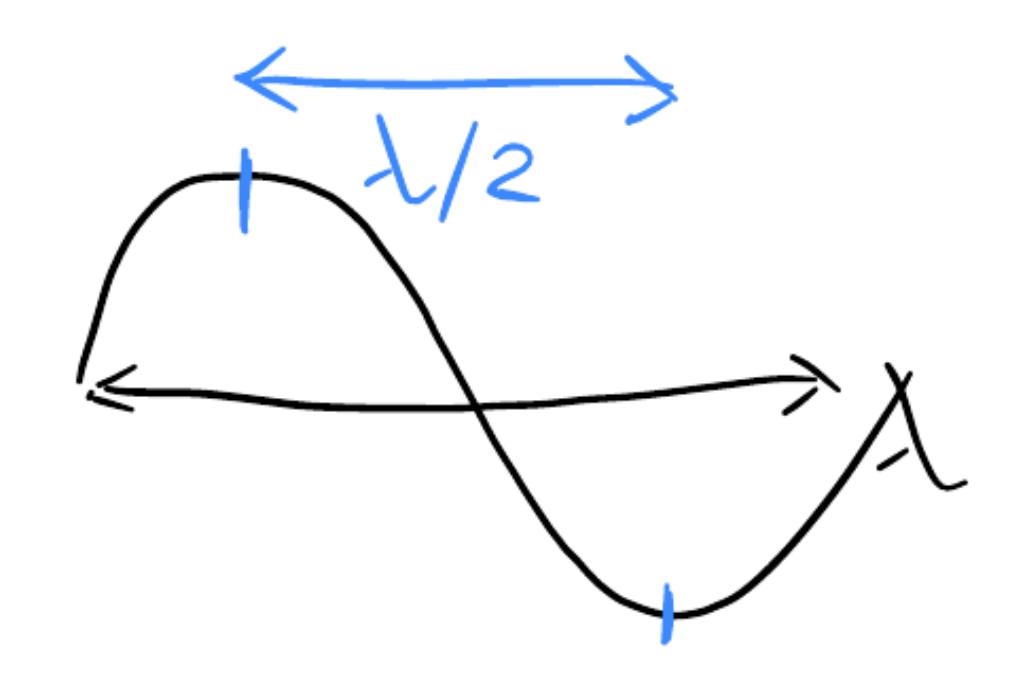
\includegraphics[width=0.5\textwidth]{Pictures/image.png}
\end{figure}

If one antenna receives the bottom, the other will receive the top.

\begin{greybox}
\faQuoteLeft \,\, Other space correlations
\end{greybox}

% PAGINA 05

\begin{greenbar}
There are other already-calculated space correlations, see \textcolor{ForestGreen}{Channel modeling (pp. 131-208), page 21}.
\end{greenbar}

\section{Time selectivity}

\subsection{Time correlation, coherence time}

What about time selectivity? We consider the case in which we have an antenna and we're moving towards the antenna or in some other direction.
We're moving and we pick various samples; we ask ourselves: are the two samples we pick in different moments correlated? Of course this depends on the velocity: depending on how fast we're going, how correlated are the signals?

Of course we have the Doppler effect. The delay between antennas is $\Delta_t = \Delta_D / v$. We find

\begin{align}
R_h(\Delta_t) = \int_{-\pi}^{\pi} \mathcal{P}(\theta) \, e^{j 2\pi f \Delta_t \cos(\theta)/c} \, d\theta \,, \tag{3.46}
\end{align}

with slight abuse of the notation $R_h(\cdot)$.

\begin{purplebox}[\faSkull \, Relation with space correlation]
If we consider

\begin{align}
R_h(\Delta_D) = \int_{-\pi}^{\pi} \mathcal{P}(\theta) \, e^{j 2\pi \Delta_D \cos(\theta)/\lambda_c} \, d\theta \,. \tag{3.42}
\end{align}

we clearly see that (3.46) is the same exact equation, just considering that:
\begin{itemize}
    \item $\Delta_D = \Delta_t v$
    \item $1/\lambda_c = f/c$.
\end{itemize}
\end{purplebox}

\begin{bluebox}[\faPen \, Coherence time]
Just like we defined $\Delta_t = \Delta_D / v$, with reference to the \textcolor{ForestGreen}{definition of coherence distance} $D_c$ we define the coherence time (the delay which should occur in order for the two replicas of a signal to be uncorrelated) as

\begin{align}
T_c = \frac{D_c}{v} \,. \tag{3.47+}
\end{align}
\end{bluebox}

From what can be gathered from exercise \textcolor{ForestGreen}{3.13}, it looks like \textbf{in a time and frequency selective channel}, we can consider the coherence time as scaled by

\[
T_c' = T_c B_c \,,
\]

with $B_c$ being the coherence bandwidth.

% PAGINA 06

\begin{greenbar}
It's clear that this makes no sense from a unit pov, but this does not stop the book from doing it!
\end{greenbar}

\section{Doppler spectrum}

As the receiver travels a distance $\Delta_D$, the length of a path at an angle $\theta$ changes by $\Delta_D \cos(\theta)$,

\begin{figure}[h]
    \centering
    % [IMAGE PLACEHOLDER: Diagram of Transmitter, Scatterer, Diffraction, Reflection, Receiver 0/1]
    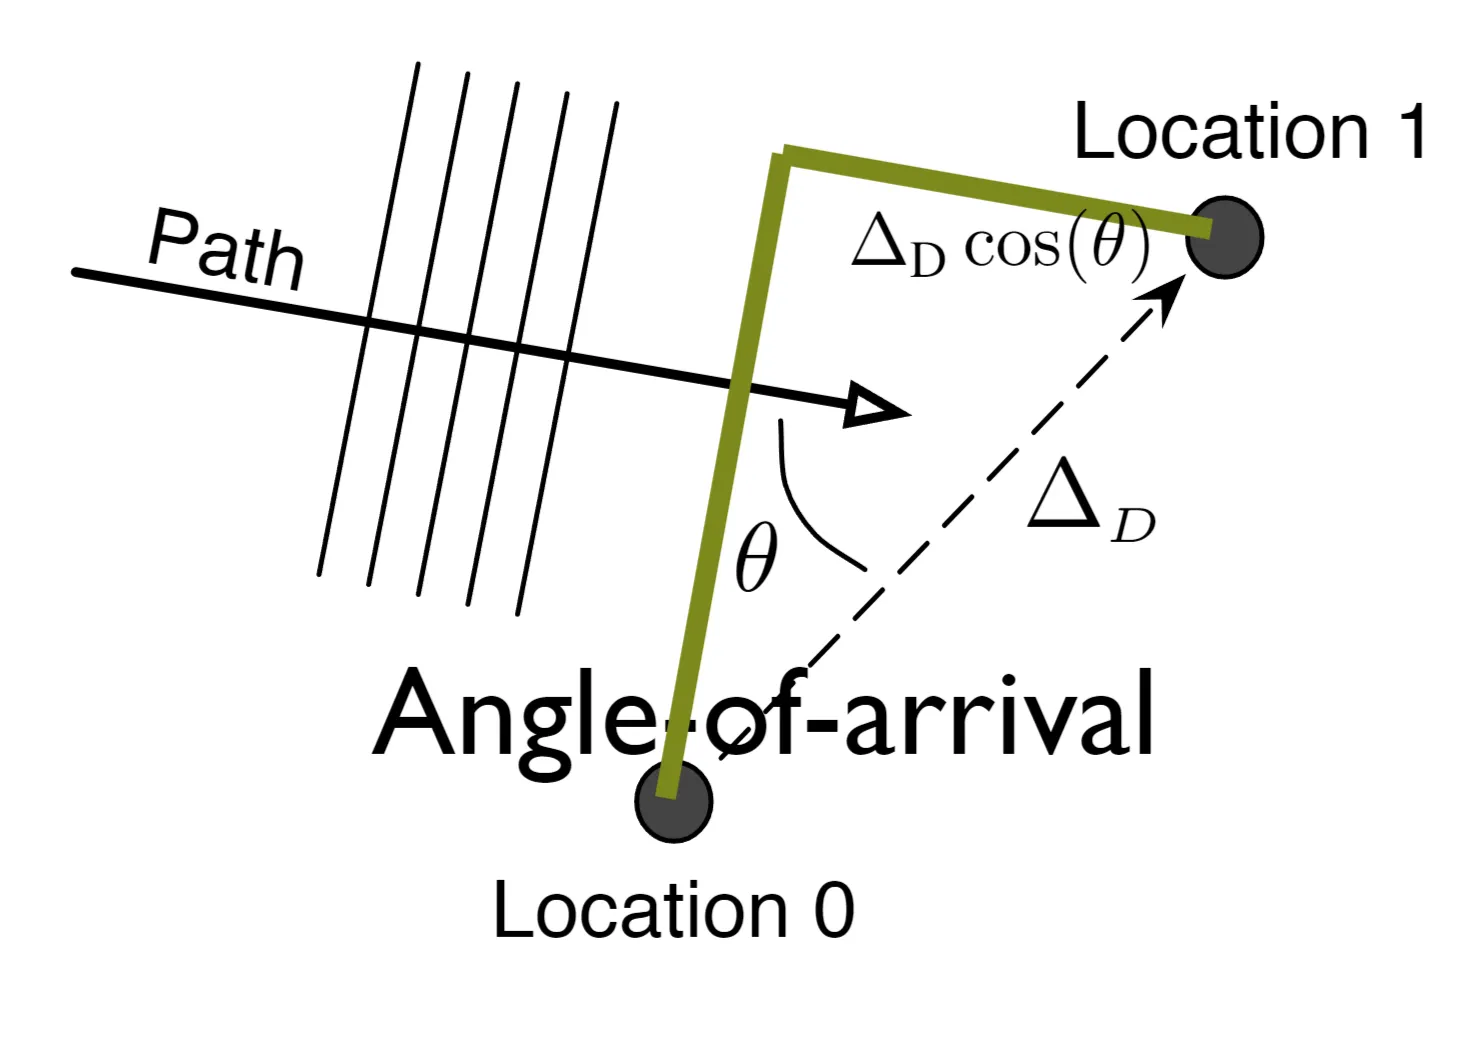
\includegraphics[width=0.5\textwidth]{Pictures/immagine-002.png}
\end{figure}

This rotates the phase of a signal at frequency $f_c$ by

\begin{align}
2\pi \Delta_D \cos(\theta) / \lambda_c \overset{\substack{\lambda_c = c/f_c \\ \Delta_D = \Delta_t v}}{=\joinrel=} 2\pi f_c \Delta_t v \cos(\theta) / c \,, \tag{*}
\end{align}

which is not different from \textcolor{ForestGreen}{what we already considered} (with the exception that now we have a moving receiver).

Since the time incurred to travel $\Delta_D$ is precisely $\Delta_t$, this phase rotation corresponds to a frequency $f_c v \cos(\theta)/c$. In other words, a signal of frequency $f_c$ arriving over a path at angle $\theta$ relative to the direction of motion \textbf{suffers a frequency increase} (which can be negative, hence a decrease) \textbf{equal to} $\nu = f_c v \cos(\theta)/c$. This frequency shift, a mere manifestation of the Doppler effect, is within the range $[-\nu_M, \nu_M]$, where

\begin{align}
\nu_M = \frac{v}{c} f_c \tag{3.48}
\end{align}

is aptly termed the \textbf{maximum Doppler shift}. Since every pair of paths at angles $\pm \theta$ map to a unique Doppler shift, (3.46) can be rewritten as an integral over Doppler shifts rather than angles.

\begin{purplebox}[{{\faSkull \, What are $f_c, v$?}}]
$v$ is the speed at which the antenna is moving, while $f_c$ is the carrier frequency.
\end{purplebox}

When we have a random process, we have correlation. Let's say we have a stationary random process; by looking at its Fourier transform, we know where the power of the
% PAGINA 07

process will be located in the frequency domain; here we do the same. We use $\nu$; this is because this is the discrete time Fourier transform! This means we're looking at the correlation in the frequency domain. What is happening is that we have a \textbf{zero outside of a certain domain} (no power outside from a certain domain): this comes from the fact that we have a bound on the speed (the speed bounds the frequency shift caused by the doppler effect). Specifically, we'll have that the correlation $R_h(\Delta_t)$ will be the Fourier antitransform of

\begin{align}
S_h(\nu) = \begin{cases}
\frac{\mathcal{P}(-\arccos(\nu/\nu_M)) + \mathcal{P}(\arccos(\nu/\nu_M))}{\sqrt{\nu_M^2 - \nu^2}} & \nu \in [-\nu_M, \nu_M] \\
0 & \nu \notin [-\nu_M, \nu_M]
\end{cases} \,. \tag{3.53}
\end{align}

\begin{purplebox}[\faGhost \, Insight!]
The idea is that $\nu/\nu_M$ should quantify the shift in a scale $\in [0,1]$, with 1 being the $2\pi$ shift; we then find the radians representation of this by using $\arccos$ and then compute $\mathcal{P}$ for the obtained value. We finally normalize over $\sqrt{\nu_M^2 - \nu^2}$.
\end{purplebox}

\begin{bluebox}[\faPen \, Doppler spectrum]
The doppler spectrum $S_h(\nu)$ for $h(\tau)$ is defined as

\begin{align*}
S_h(\nu) = \mathcal{F}[R_h(\Delta_t)] = \int_{-\infty}^{+\infty} R_h(\Delta_t) e^{-j 2\pi \nu \Delta_t} \, dx \,.
\end{align*}

\begin{greenbar}
This is a sort of re-interpretation of (3.51)
\end{greenbar}
\end{bluebox}

Doppler spectrum can be interpreted as follows: a transmit sinusoid of frequency $f_c$ gets smeared into received components at every frequency within $[f_c - \nu_M, f_c + \nu_M]$ as indicated by $S_h(\nu)$. As can be verified, we have

\begin{align}
\int_{-\pi}^{\pi} \mathcal{P}(\theta) \, d\theta = \int_{-\nu_M}^{\nu_M} S_h(\nu) \, d\nu \,. \tag{3.54}
\end{align}

Professor does not want us to remember (3.53). Instead, we need to remember the shape of this value, which is the \textbf{Clarke-Jakes Doppler spectrum}:


% PAGINA 08

\begin{figure}[h]
    \centering
    % [IMAGE PLACEHOLDER: Diagram of Transmitter, Scatterer, Diffraction, Reflection, Receiver 0/1]
    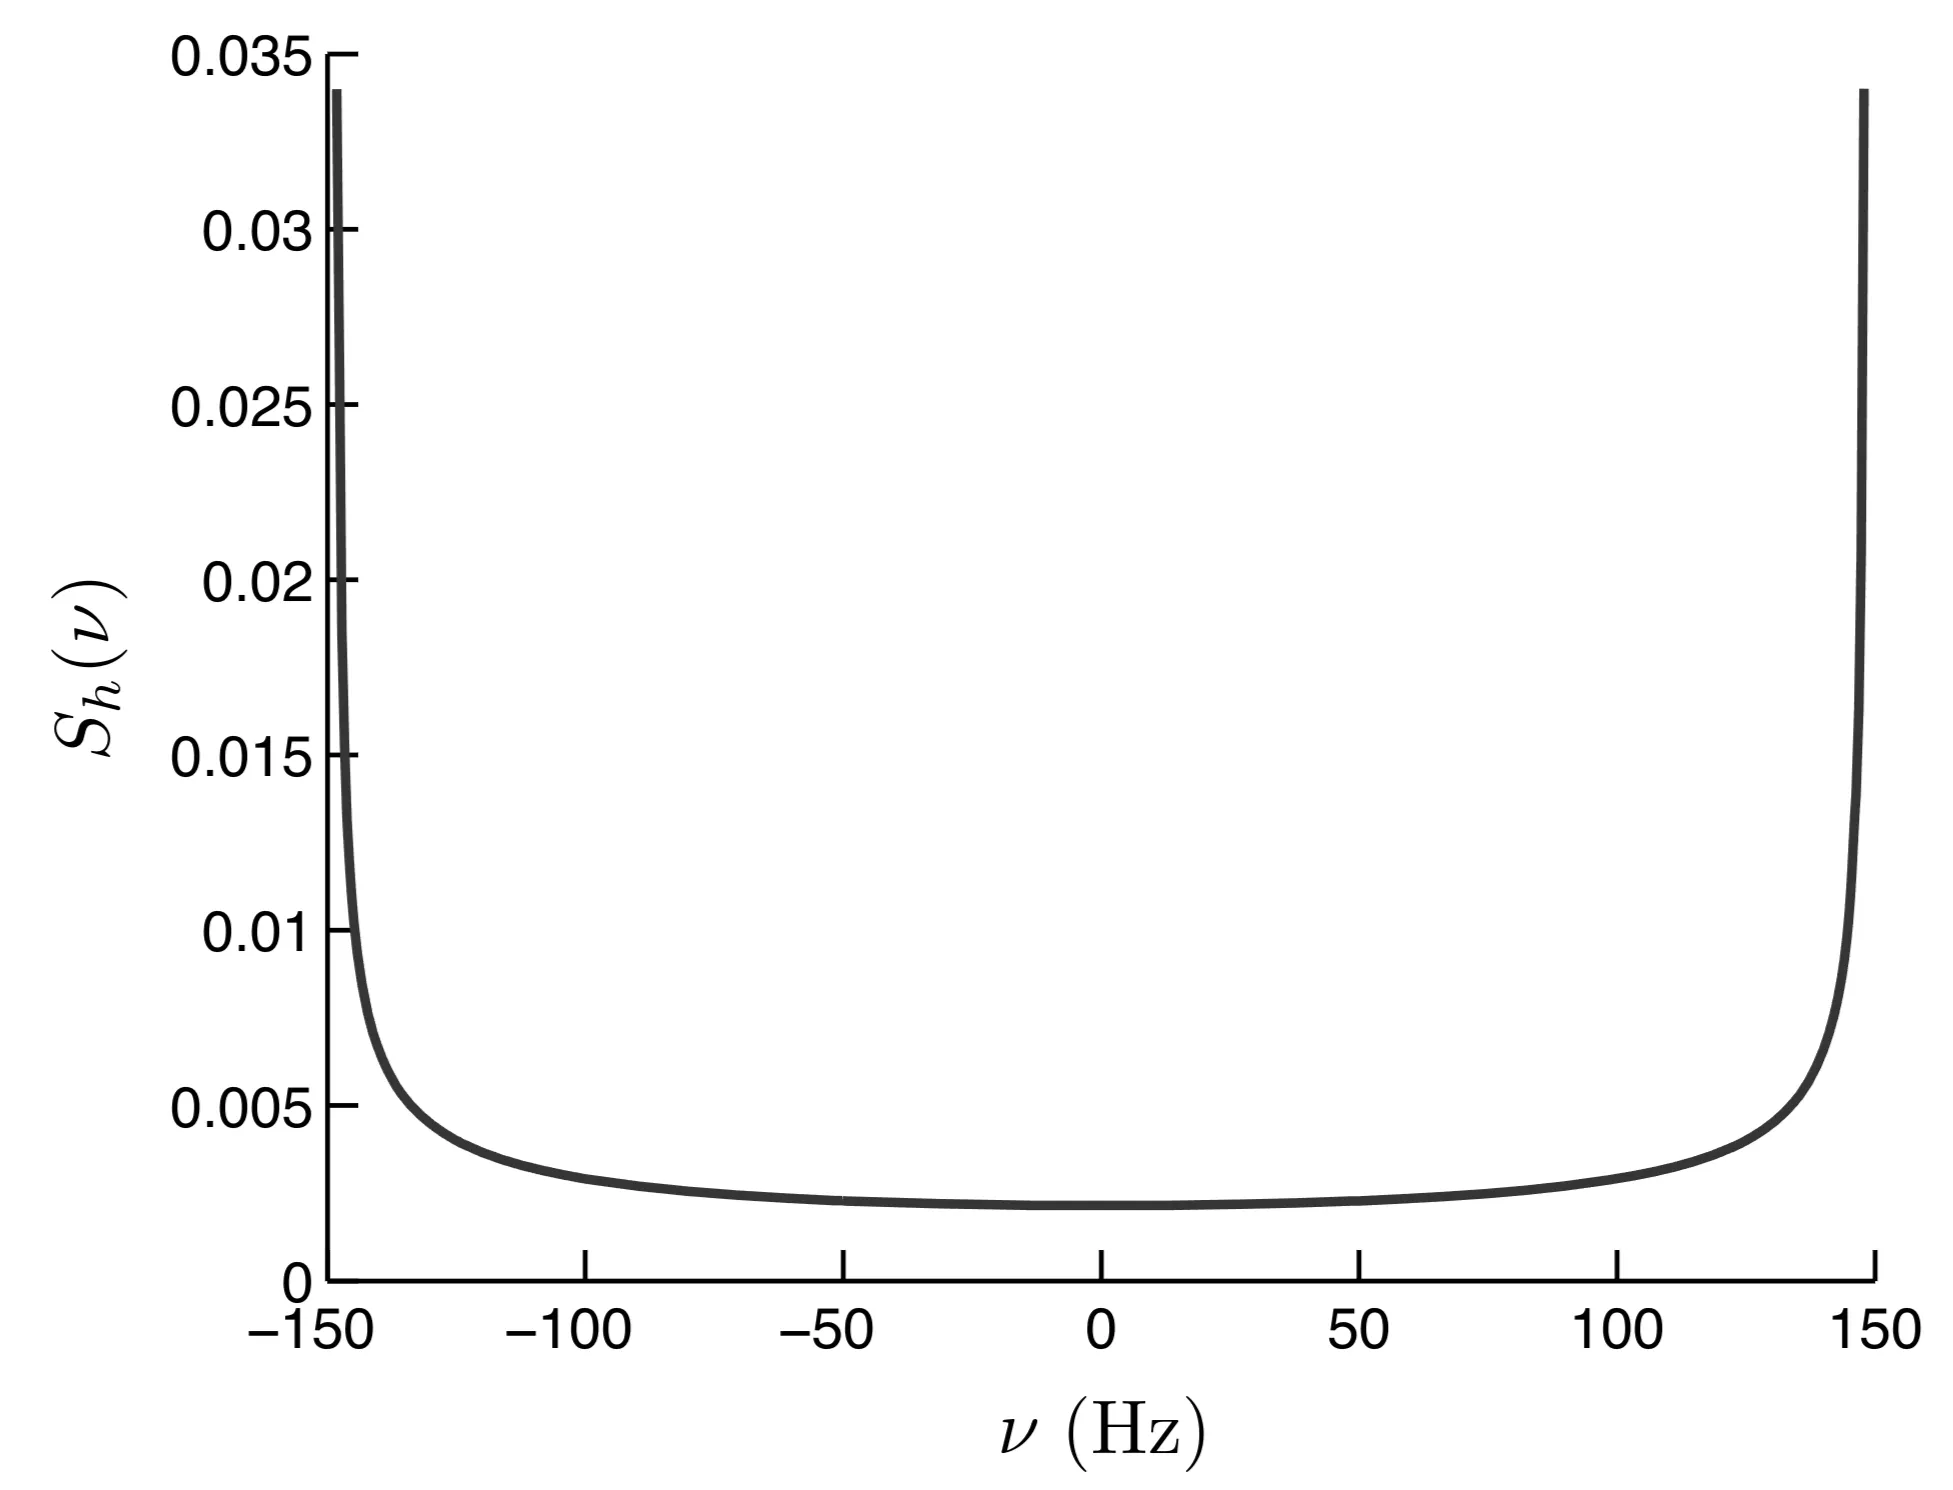
\includegraphics[width=0.5\textwidth]{Pictures/immagine-003.png}
\end{figure}

This is for $\nu_M = 148\text{GHz}$, which (for example) corresponds to $v = 80\text{km/h}$ at $f_c = 2\text{GHz}$.

It goes to $\infty$ at the extremis.
If we're at 0, we have little energy; this means that the process is low energy in that part: this means that it's stable, it does not move. We have more energy towards higher spectrum, higher Doppler. \textbf{That's where we have more chance to have higher independence}.

\begin{greenbar}
The higher the frequency, the lower the correlation.
If we don't move, the signal will be the same when we start and when we end. If we're really fast, the signal will be really different.
\end{greenbar}

\begin{purplebox}[\faSkull \, Clarke-Jakes PAS]
It's really not that hard to find the Doppler Spectrum for the Clarke-Jakes PAS.
From (3.53), we just have

\[
S_h(\nu) = \begin{cases}
\frac{\frac{1}{2\pi} + \frac{1}{2\pi}}{\sqrt{\nu_M^2 - \nu^2}} & \nu \in [-\nu_M, \nu_M] \\
0 & \text{Otherwise}
\end{cases} \,.
\]

This has a clear graph of

\begin{center}
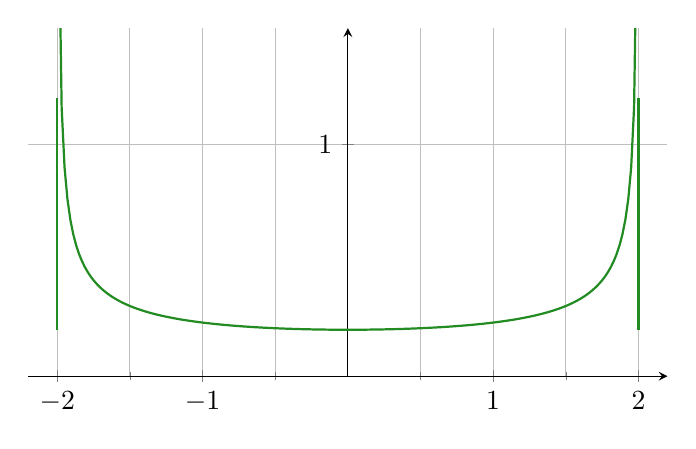
\begin{tikzpicture}
    \begin{axis}[
        width=0.8\linewidth,
        height=6cm,
        axis lines=middle,
        xmin=-2.2, xmax=2.2,
        ymin=0, ymax=1.5,
        xtick={-2, -1, 0, 1, 2},
        ytick={1},
        grid=both,
        major grid style={line width=.2pt,draw=gray!50},
        minor tick num=1,
        samples=200,
        domain=-1.99:1.99
    ]
        \addplot [thick, ForestGreen] {0.4 / sqrt(4 - x^2)};
        
        % Asymptotes
        \draw[thick, color=ForestGreen] (axis cs:-2, 0.2) -- (axis cs:-2, 1.2);
        \draw[thick, color=ForestGreen] (axis cs:2, 0.2) -- (axis cs:2, 1.2);
    \end{axis}
\end{tikzpicture}
\end{center}

Which here is plotted for $\nu_M = 2$.
\end{purplebox}

% PAGINA 09

This depends on signal and carrier; when we have a low carrier, if we move 1m nothing changes, because the carrier is having a long wavelength.

Here we're considering \textit{nonregular fading}, which:

\begin{itemize}
    \item Comes from the assumption that a signal can bounce only once from an object
    \item Makes it so that $S_h(\cdot)$ has a bandlimited nature which allows us to predict the present value in a deterministic manner, given that noiseless observations of the whole past are available.
\end{itemize}

If we get rid of the \textit{one-bounce} assumption, then we get doppler shifts larger than $\nu_M$ and that the present value cannot be predicted from observations of past values. This is called \textit{regular fading}.

\begin{yellowbox}[\faLink \, Channel modeling (pp. 131-208), page 26]
Unless otherwise stated, we consider nonregular fading bandlimited to $\nu_M$. While Doppler shifts exceeding this value are possible, the corresponding signal components are likely to be very weak relative to those within $[-\nu_M, \nu_M]$ and hence, barring exceedingly high SNRs, those components beyond $\pm \nu_M$ are likely to be buried well below the noise level.
\end{yellowbox}

\section{Time discretization: time selectivity applied to discrete transmission}

\begin{yellowbox}[\faLink \, Channel modeling (pp. 131-208), page 26]
For fading conforming to $h(t, \tau) = h(t)\delta(\tau)$ as we are considering thus far, the channel has the multiplicative effect $y(t) = \sqrt{G} h(t) x(t)$ and, as we learned in Example 2.3, the sampled pseudo-baseband gain $h[n] = h(nT)$ suffices for a discrete-time representation; we can directly write $y[n] = \sqrt{G} h[n] x[n]$. Strictly speaking, the time-discretization of $y(t)$ should entail a sampling period $\frac{1}{B + \nu_M}$ because the bandwidth $B$ of the transmit signal increases to $B + \nu_M$ as \textbf{the signal undergoes time-varying fading}.
\end{yellowbox}

\begin{purplebox}[\faSkull \, About the enlargement of bandwidth]
From what I understand, the bandwidth of $[-\nu_M, \nu_M]$ only holds for a complex exponential; if we have a real signal of bandwidth $B$, we'll need to have $\nu_M$ before and after that bandwidth, as we can consider each slice of band as a complex exponential.
\end{purplebox}

Up to now, we've been in the continuous time domain. If we want to go to the discrete time domain, we want to sample the signal.
We have a signal which no longer could very well not be an exponential at this point; it has a certain bandwidth which we'll sample with the inverse of that bandwidth.
This is not mathematically complete. We might actually have a bandwidth which goes
% --- PAGINA 10 ---

from $B + \nu_M$ to $-B - \nu_M$, with

\begin{align}
\nu_M = \frac{v}{c} f_c \tag{3.48}
\end{align}

\begin{figure}[h]
    \centering
    % [IMAGE PLACEHOLDER: Diagram of Transmitter, Scatterer, Diffraction, Reflection, Receiver 0/1]
    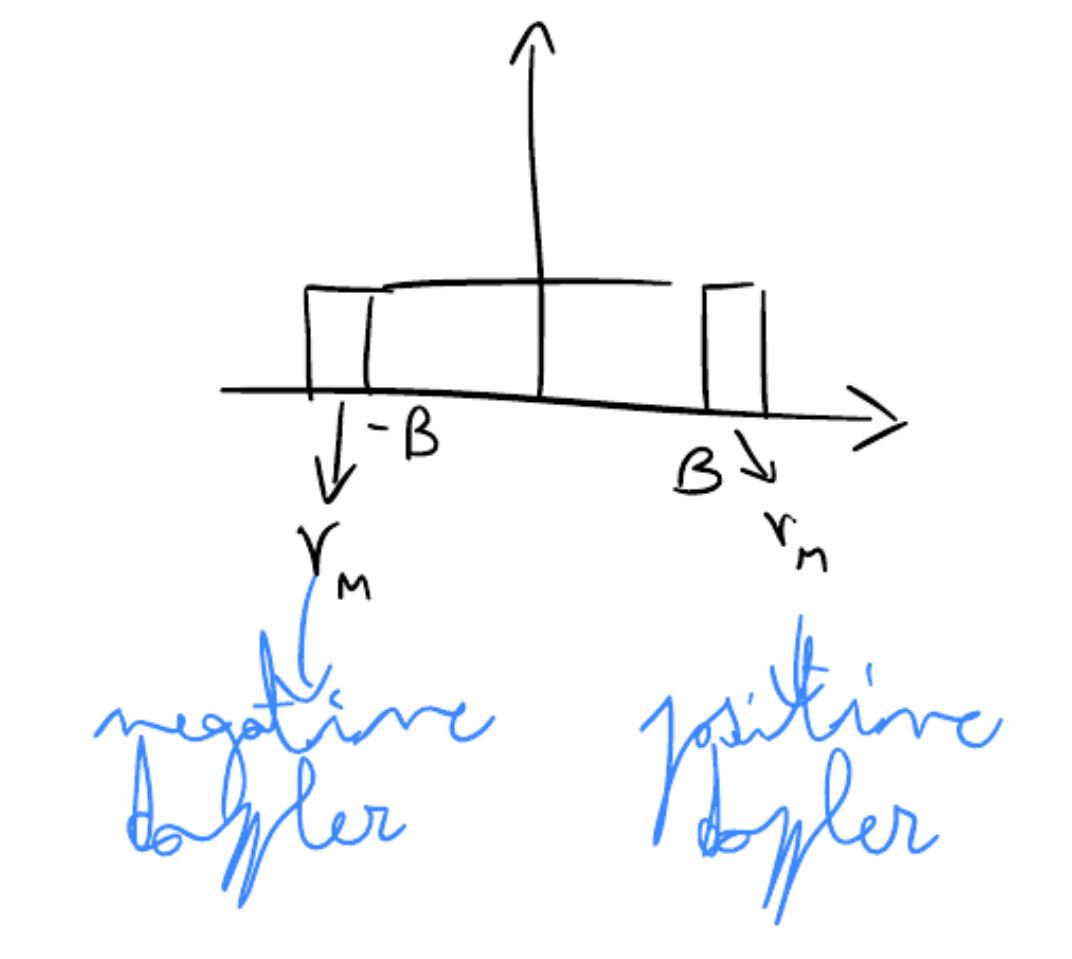
\includegraphics[width=0.5\textwidth]{Pictures/image copy.png}
\end{figure}

We can have another approximation, aka that $\nu_M \ll B$: if they were comparable, we should sample at a higher sampling rate. Even if $\nu_M$ is very small, we still violate the Nyquist principle; point is that if we actually have $\nu_M \ll B$, we'll have a small loss even if we sample with $B=1/T$.
Also, normally signals don't really have a specific spectrum; if we have a specific spectrum, we have something more in the lines of a rcos and such.
We should not forget $\nu_M \ll B$ because of the concept; \textbf{what's really important is to have a Time-varying flat-fading model}. If we take a large $B$ but the channel has many taps (delays), then we'll have a frequency-selective channel.

Since $h[n] = h(nT)$, we'll equivalently have that \textbf{the autocorrelation of $h[n]$ equals $R_h(\ell T)$, where $R_h(\tau)$ is the autocorrelation of $h(t)$.}

Given $S_h(\nu)$ (aka the Doppler spectrum of $h(t)$), the Doppler spectrum of $h[n]$ equals

\begin{align}
\frac{1}{T} S_h \left( \frac{\nu'}{T} \right) \,, \quad \nu' \in [-\nu_M T, \nu_M T] \tag{3.60}
\end{align}

with the factor $1/T$ ensuring that the scaling of the frequency axis $\nu$ to $\nu' = \nu T$ does not affect the power.

\begin{greenbar}
The book uses a different notation, but I can't seem to find the specific font setting to have that $\nu$.
\end{greenbar}

The book is looking at the different aspects one at a time; now it looks at how flat channels are correlated in time and then correlation in frequency. At the end of the day, all of this converges together.
When we send $x[n]$, we have a different $h[n]$: this is a problem if we need to estimate it!


% --- PAGINA 11 ---

If every symbol has a different channel, it's impossible to communicate; oc this is not the case, otherwise we wouldn't be able to transmit.

\begin{greenbar}
There are models doing this using AI or neural networks.
\end{greenbar}

It might also be relevant to know that for a frequency-flat channel (which might very well hold also for just a complex exponential in whichever channel), we have

\begin{align}
T_c \approx \frac{1}{2\nu_M} \tag{3.59}
\end{align}

\section{Simplified models}

\subsection{Why do we need simplified models?}

\begin{yellowbox}[\faLink \, 08.3 Channel modeling (pp. 131-208), page 27]
As mentioned at the outset of the chapter, the art of channel modeling must seek a \textbf{compromise between realism and tractability}, distilling what is essential for each purpose. When it comes to fading dynamics, it is sometimes desirable to have models that capture the essence of time selectivity but are otherwise stripped down to the bones. We next introduce two such models, formulated directly for the discrete-time complex channel
\end{yellowbox}

\section{Gauss-Markov model}

A first possibility is to resort to a first-order Gauss-Markov process, or first-order autoregressive process, whereby the fading at symbol $n$ satisfies

\begin{align}
h[n] = \sqrt{1 - \epsilon} h[n-1] + \sqrt{\epsilon} w[n] \,, \tag{3.61}
\end{align}

where $\{w[n]\}$ is a sequence of IID random variables with $w \sim \mathcal{N}_{\mathbb{C}}(0,1)$.

In turn, $\epsilon$ is the one-step prediction error, i.e. the variance of the error to which $h[n]$ can be predicted from a noiseless observation of $h[n-1]$, something that in a first-order Markov process is as informative as a noiseless observation of the entire past. By definition, a Gauss-Markov process is regular and its degree of decorrelation after $\ell$ symbols is determined by $\epsilon$ via

\begin{align}
R_h[\ell] &= \mathbb{E}[h[n]h^*[n+\ell]] \tag{3.62} \\
&= (1 - \epsilon)^{\ell/2} \,. \tag{3.63}
\end{align}

What people sometimes do is to say \textit{the next channel is the previous channel with a factor $\sqrt{1-\epsilon}$ and since we want to make it random, we add a bit of noise, $w[n]$}.
This is a random path: the channel is changing but not too much, because in the ingredients we have a predictable part and also some noise.
This is called Gauss-Markov model. The correlation here is $(1-\epsilon)^{\ell/2}$, where $l$ is the distance between the sampling of the channel.
If we have $\epsilon \to 0$, the channel is completely stable.

\section{Block-fading model}

% --- PAGINA 12 ---

\begin{tcolorbox}[colback=white, colframe=red!80!white, title=\textbf{\faBomb \, Might not be in the exam}, fonttitle=\bfseries\color{red!80!white}, coltitle=red!80!white, attach boxed title to top left={yshift=-2mm, xshift=2mm}, boxed title style={colback=white, frame hidden}, sharp corners]
Although professor is a madlad and might ask this no matter what, this is not in the course programme!
\end{tcolorbox}

A second possibility, illustrated in Fig. 3.12, is to resort to a block-fading structure, whereby the \textbf{fading remains constant over blocks of duration $T_c$} while changing values across blocks. It is worth noting that this model is not stationary but rather \textbf{cyclostationary with period $T_c$}. The fading values at consecutive blocks may be correlated, but are most often assumed IID.

\begin{center}
\begin{tikzpicture}[scale=1.2]
    % Axes
    \draw[->] (0,0) -- (6,0) node[right] {$t$};
    \draw[->] (0,0) -- (0,2.5) node[left] {$|h|$};
    
    % Steps
    \draw[thick] (0.2, 1.2) -- (1, 1.2) -- (1, 0.8) -- (2, 0.8) -- (2, 1.0) -- (2.5, 1.0) -- (2.5, 1.9) -- (3, 1.9) -- (3, 1.2) -- (3.5, 1.2) -- (3.5, 0.3) -- (4, 0.3) -- (4, 0.8) -- (4.5, 0.8) -- (4.5, 1.5) -- (5, 1.5) -- (5, 1.0) -- (5.5, 1.0);
    
    % Tc marking
    \draw[<->] (3.5, 0.2) -- (4, 0.2) node[midway, below] {$T_c$};
    
    % Figure Label
    \node at (3, -0.8) {\small Figure 3.12};
\end{tikzpicture}
\end{center}

If $N_c$ is the number of single-carrier symbols (where the single-carrier bit is specified only to allow us to apply the results which we saw for single carrier cases) we have per block, we have that

\begin{align}
N_c &= \frac{T_c}{T} \tag{3.65} \\
&= B T_c \tag{3.66}
\end{align}

and, if the blocks are IID, then it makes sense to set $T_c$ to coincide with the \textbf{coherence time of a stationary process}. Recalling (3.59), which says that $T_c = 1/2\nu_M$, this leads to

\begin{align}
N_c = \frac{1}{2 \nu_M T} \,. \tag{3.67}
\end{align}

\begin{yellowbox}[\faLink \, 08.3 Channel modeling (pp. 131-208), page 28]
However, care must be exercised with both (3.66) and (3.67) because they \textbf{hold only if the bandwidth $B$ is "not too large"} where the precise meaning of "not too large" is to become clear in the next section.

\begin{greenbar}
They are most likely referring to the coherence bandwidth concept.
\end{greenbar}

The block-fading model can be broadened to allow for continuous variability within each block, with transitions to independent values across blocks. This more general blockfading model can sometimes serve as a convenient bridge with a true continuous fading model [245, 246].
\end{yellowbox}

We have jumps in time: we know that the signal has infinite bandwidth.
We now go and look at how the frequency response of the channel is changing.
This is called \textit{block fading model}: at every symbol it looks like we have fading, a jump.
We know this does not actually happen, in fact this is a model.
\begin{greenbar}
This is not a coherent theory, it's just an excursus of various channel models.
\end{greenbar}

Yesterday we stopped at the block fading channel. We've seen this is a simplified model which is quite used. The problem is setting $\epsilon$.
Clearly deciding what to set it to is a problem.
\end{document}

